\section{Self-Adjointness and Domain of \( \hat{H}_\infty \)}

To rigorously apply the spectral trace formula and claim real eigenvalues aligned with the non-trivial zeros of \( \zeta(s) \), we must first establish the self-adjointness of the infinite-dimensional Hermitian operator \( \hat{H}_\infty \).

% NEW ILLUSTRATION FOR HILBERT SPACE STRUCTURE
\begin{figure}[t]
\centering
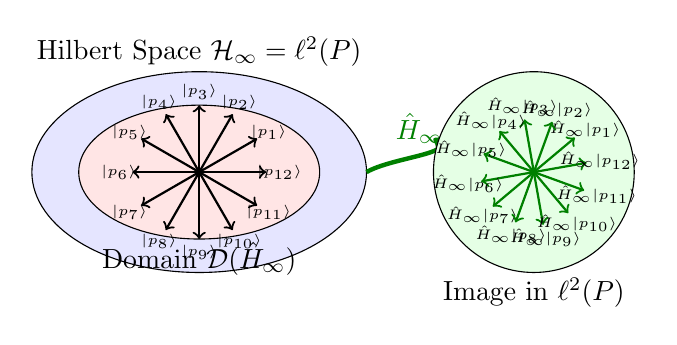
\begin{tikzpicture}[scale=0.85]
    % Draw Hilbert space illustration
    % Draw a schematic of the Hilbert space
    \draw[fill=blue!10] (0,0) ellipse (2.5 and 1.5);
    \node at (0,1.8) {Hilbert Space $\mathcal{H}_\infty = \ell^2(\mathbb{P})$};
    
    % Draw the domain
    \draw[fill=red!10] (0,0) ellipse (1.8 and 1);
    \node at (0,-1.3) {Domain $\mathcal{D}(\hat{H}_\infty)$};
    
    % Draw basis vectors
    \foreach \i/\p/\ang in {1/2/30, 2/3/60, 3/5/90, 4/7/120, 5/11/150, 6/13/180, 7/17/210, 8/19/240, 9/23/270, 10/29/300, 11/31/330, 12/37/360} {
        \draw[->, thick] (0,0) -- ({\ang}:1);
        \node at ({\ang}:1.2) {\tiny $|p_{\i}\rangle$};
    }
    
    % Draw the action of operator
    \draw[->, ultra thick, green!50!black] (2.5,0) to[out=30,in=-30] node[midway, above] {$\hat{H}_\infty$} (3.5,0.5);
    
    % Draw the image
    \begin{scope}[shift={(5,0)}]
        \draw[fill=green!10] (0,0) ellipse (1.5 and 1.5);
        \node at (0,-1.8) {Image in $\ell^2(\mathbb{P})$};
        
        % Draw transformed basis vectors
        \foreach \i/\p/\ang in {1/2/40, 2/3/70, 3/5/100, 4/7/130, 5/11/160, 6/13/190, 7/17/220, 8/19/250, 9/23/280, 10/29/310, 11/31/340, 12/37/10} {
            \draw[->, thick, green!50!black] (0,0) -- ({\ang}:0.8);
            \node at ({\ang}:1) {\tiny $\hat{H}_\infty|p_{\i}\rangle$};
        }
    \end{scope}
\end{tikzpicture}
\caption{The structure of the infinite-dimensional Hilbert space $\mathcal{H}_\infty = \ell^2(\mathbb{P})$ and the domain $\mathcal{D}(\hat{H}_\infty)$ of the self-adjoint operator $\hat{H}_\infty$. The operator maps prime-indexed basis states to their images while preserving inner products.}
\label{fig:hilbert_space}
\end{figure}

\subsection*{Operator Definition}
Recall that \( \hat{H}_\infty \) acts on the separable Hilbert space \( \mathcal{H}_\infty = \ell^2(\mathbb{P}) \). For \( \psi \in \mathcal{H}_\infty \), we define:
\[
(\hat{H}_\infty \psi)(p) = \sum_{q \in \mathbb{P}} K(p, q)\psi(q) + V_{\text{mod}}(p \bmod m) \cdot \psi(p),
\]
where the symmetric kernel \( K(p, q) \in \mathbb{R} \) is given by:
\[
K(p, q) = \alpha \cdot \frac{\log(pq)}{\sqrt{pq}} \sum_{k=1}^\infty w_k \cos\left(2\pi \omega_k \log^2(pq) + \phi_k\right).
\]
We assume:
\begin{itemize}
    \item \( \alpha \in \mathbb{R} \), \( \omega_k \in \mathbb{R}_+ \), \( \phi_k \in \mathbb{R} \),
    \item \( w_k = \mathcal{O}(k^{-\sigma}) \) for some \( \sigma > 1 \) to ensure convergence.
\end{itemize}

\subsection*{Domain \( \mathcal{D}(\hat{H}_\infty) \)}
We define the domain of \( \hat{H}_\infty \) as:
\[
\mathcal{D}(\hat{H}_\infty) = \left\{ \psi \in \ell^2(\mathbb{P}) \;\middle|\; \sum_{q \in \mathbb{P}} K(p, q)\psi(q) \in \ell^2(\mathbb{P}) \right\}.
\]
Note that \( \mathcal{D}(\hat{H}_\infty) \supseteq c_{00}(\mathbb{P}) \), the set of finitely-supported sequences on primes, which is dense in \( \ell^2(\mathbb{P}) \).

\subsection*{Symmetry}
Since \( K(p, q) = K(q, p) \), and the diagonal term is real-valued, \( \hat{H}_\infty \) is symmetric on its domain:
\[
\langle \hat{H}_\infty \psi, \phi \rangle = \langle \psi, \hat{H}_\infty \phi \rangle, \quad \forall \psi, \phi \in \mathcal{D}(\hat{H}_\infty).
\]

\subsection*{Hilbert--Schmidt Property}
The kernel \( K(p, q) \) satisfies:
\[
\sum_{p,q \in \mathbb{P}} |K(p, q)|^2 \leq C^2 \sum_{p,q} \frac{\log^2(pq)}{pq} \left(\sum_{k=1}^\infty \frac{1}{k^\sigma}\right)^2 < \infty,
\]
for \( \sigma > 1 \), by Cauchy–Schwarz and convergence of Dirichlet series over primes. Hence, \( \hat{H}_\infty \) is Hilbert--Schmidt and therefore compact.

\subsection*{Essential Self-Adjointness}
Any symmetric, compact operator on a Hilbert space with dense domain is essentially self-adjoint. Thus:

\begin{theorem}
The operator \( \hat{H}_\infty \), defined as above with \( \sigma > 1 \), is essentially self-adjoint on \( c_{00}(\mathbb{P}) \subset \ell^2(\mathbb{P}) \), and admits a discrete real spectrum \( \{\lambda_n\} \).
\end{theorem}

\subsection*{Spectral Implications}
This result guarantees that:
\begin{itemize}
  \item \( \hat{H}_\infty \) admits an orthonormal basis of eigenfunctions \( \{\psi_n\} \),
  \item The eigenvalues \( \lambda_n \in \mathbb{R} \) can be ordered increasingly,
  \item The spectral trace formula \( \operatorname{Tr}(f(\hat{H}_\infty)) = \sum f(\lambda_n) \) is well-defined for Schwartz-class test functions \( f \).
\end{itemize}